% By SharkD (Own work) [GFDL (http://www.gnu.org/copyleft/fdl.html) or
% CC BY-SA 4.0-3.0-2.5-2.0-1.0
% (http://creativecommons.org/licenses/by-sa/4.0-3.0-2.5-2.0-1.0)], via
% https://commons.wikimedia.org/wiki/File:RGB_farbwuerfel.jpg
% Wikimedia Commons
% http://www.scratchapixel.com/old/lessons/3d-basic-lessons/lesson-5-colors-and-digital-images/color-spaces/

\section{Représentation informatique d'une couleur}
Commençons par parler de couleur. Il s'agit, comme toujours en
informatique, de décider de la façon de stocker l'information
«~couleur~».

On peut choisir d'utiliser 1~bit pour stocker cette
information. On distinguera alors uniquement deux couleurs. Par
exemple du noir (0) et du blanc (1) ou alors du blanc (0) et du noir
(1) ou pourquoi pas du rouge et du noir. 

On peut choisir d'utiliser 1~octet pour stocker cette information. On
distinguera alors $2^8=256$ couleurs différentes. Ces $256$ valeurs
différentes peuvent représenter des niveaux de gris différents (du
blanc au noir ou alors du noir au blanc) ou pourquoi pas du blanc au
rouge en passant par 254 nuances de rose.

Le plus souvent, on utilise 3~octets pour stocker une couleur. On distingue
alors $256^3 = 16\,777\,216$ couleurs différentes. La norme RGB consiste à
séparer ces trois octets et les penser comme
 un vecteur à 3~coordonnées dans l'espace
$R\times G \times B$, où chaque coordonnée peut prendre $2^8=256$
valeurs. 

\renewcommand{\figurename}{}
\renewcommand{\thefigure}{}
\begin{figure}[h]
  \centering
  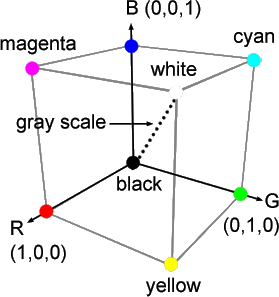
\includegraphics[width=.45\textwidth]{../input_exos_python/theme_image_1_fig_1}
  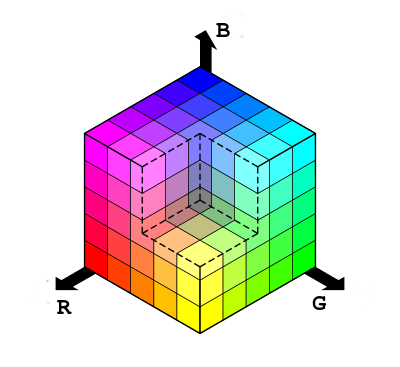
\includegraphics[width=.45\textwidth]{../input_exos_python/theme_image_1_fig_2}
  \caption{\ccbysa\ }
  % \caption{By SharkD (Own work), \ccbysa\ }
  % https://commons.wikimedia.org/wiki/File:RGB_color_solid_cube.png
\end{figure}

On peut aussi utiliser 4~octets (trois octets pour la couleur et un
pour la transparence).

On peut aussi utiliser des résolutions plus importantes, des
compressions sans pertes. 

Bref, il importe de se référer aux spécifications des fichiers que l'on
utilise~!

\section{Représentation informatique d'une image}

% Nous ne nous intéressons pas ici à la représentation vectorielle des
% images, qui consiste à décrire la construction mathématique d'une
% image. Nous ne nous intéressons pas non plus aux formats compressés
% des images. 
Il existe de nombreuses façons de représenter informatiquement une
image. Certaines sont vectorielles (SVG, PS), compressées (JPG) d'autres
matricielles (PNG). Nous ne nous intéressons ici qu'aux images au
format PNG. Il s'agit d'un ensemble
discret de points ayant chacun une couleur donnée. Ces points
s'appellent des pixels. La résolution de
l'image dépend du nombre de points (nombre de lignes et de colonnes),
et aussi du nombre de bits servant à coder les couleurs.

Une image est stockée dans un tableau numpy, dont le
\texttt{shape} est \texttt{(n,p,3)}, avec $n$ le nombre de lignes, $p$
le nombre de colonnes et $3$ le nombre d'octets pour coder les
couleurs. 

% Le \texttt{dtype} des images que nous utilisons ici est
% \texttt{float32}. 

En plus des bibliothèques habituelles
\begin{python}
import numpy as np
import matplotlib.pyplot as plt
\end{python}
on charge la bibliothèque~:
\begin{python}
import matplotlib.image as mpimg
\end{python}
qui nous permet d'utiliser les instructions~: 
\begin{itemize}
\item 
  \verb#img = mpimg.imread(filename)#~: le fichier PNG \verb#filename#
  est converti en tableau numpy et nommé \verb#img#.
\item 
  \verb#plt.imshow(img)#~: comme \verb#plt.plot(...)#, l'affichage de
  \verb#img# est préparé, et sera utilisé par \verb#plt.show()# ou
  \verb#plt.savefig(filename2)#.
\item
  \verb#mpimg.imsave(filename2, img)# permet d'enregistrer l'image
  (qui n'est pas un schéma python, n'a pas d'axes, de titre etc.)
\end{itemize}

\begin{remark}
  Avec \texttt{matplotlib.image}, les tableaux numpy sont de
  \texttt{dtype} \texttt{float32}, mais ils sont constitués uniquement
  de 256 valeurs flottantes uniformément réparties entre $0$ et $1$.
\end{remark}


\section{Manipulation d'images}

\begin{enumerate}
\item 
  Télécharger les deux fichiers PNG \texttt{playmobil.png} et
  \texttt{montagne.png} sur le site de la classe. Les
  ouvrir avec \texttt{matplotlib.image.imread} et les afficher.\\
  L'objectif de cet exercice est d'incruster le paysage de montagne
  derrière les Playmobil\textsuperscript{\textregistered}.

\begin{figure}[h]
  \centering
  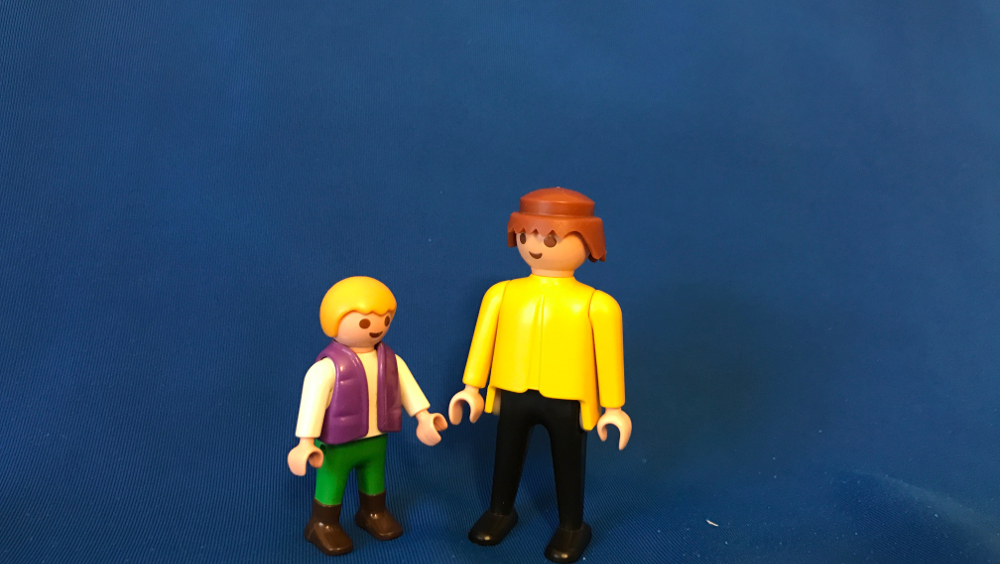
\includegraphics[width=.45\textwidth]{../input_exos_python/theme_image_1_playmobil}
  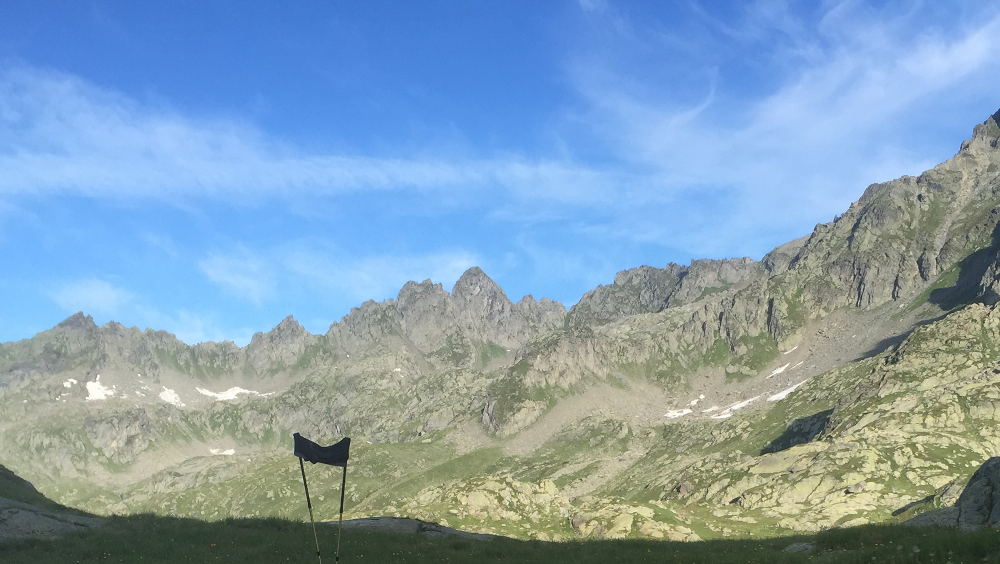
\includegraphics[width=.45\textwidth]{../input_exos_python/theme_image_1_montagne}
\end{figure}

\item 
  Déterminer pour l'image \texttt{playmobil.png}~: la taille, le
  \texttt{dtype}, la couleur du  pixel en position (300,300) et les
  valeurs max. et min. des éléments. 
  % Quelle est la taille théorique du fichier~?

\item 
  Est-ce que le fond bleu est de couleur uniforme~?

% \item 
%   Définir une fonction \verb#distance(u,v)# prenant en argument deux
%   vecteurs représentés par des tableaux numpy unidimensionnels, et qui
%   renvoie la distance euclidienne entre ces deux vecteurs.

\item
  En sélectionnant par exemple les pixels dont la couleur est à une
  distance euclidienne faible d'un pixel de référence, «~supprimer~»
  le fond bleu de l'image \texttt{playmobil}. \\
  De même, «~supprimer~» de
  l'image \texttt{montagne} les pixels correspondant aux personnages.\\
  Construire alors l'image représentant les personnages devant la
  montagne. 

\item
  Enregistrer cette nouvelle image au format PNG. 

\end{enumerate}
